\subsection{Overview}

The high-level architectural diagram provided below offers a conceptual overview of the CodeKataBattle (CKB) platform's infrastructure. It delineates the system's division into three primary layers: Presentation, Application, and Data. 

The Presentation Layer captures the user interaction with the system via a standard web browser, illustrating the entry point for both educators and students. 

The Application Layer is the system's backbone, housing the business logic and core functionalities, including load balancing, application servers, and interfaces for external services such as the GitHub API, Static Analysis Tool API, Email Service, and Notification Service. A dedicated firewall protects this layer, ensuring secure data transactions. 

The Data Layer is structured to manage persistent data and comprises the Database Management System (DBMS), which supports sharded databases for scalability, and a File Storage system that accommodates various data types, including educator uploads and code submissions. 

Each component is strategically placed to optimize performance and maintainability, reinforcing the platform’s robustness and reliability.

\begin{figure}[H]
    \centering
    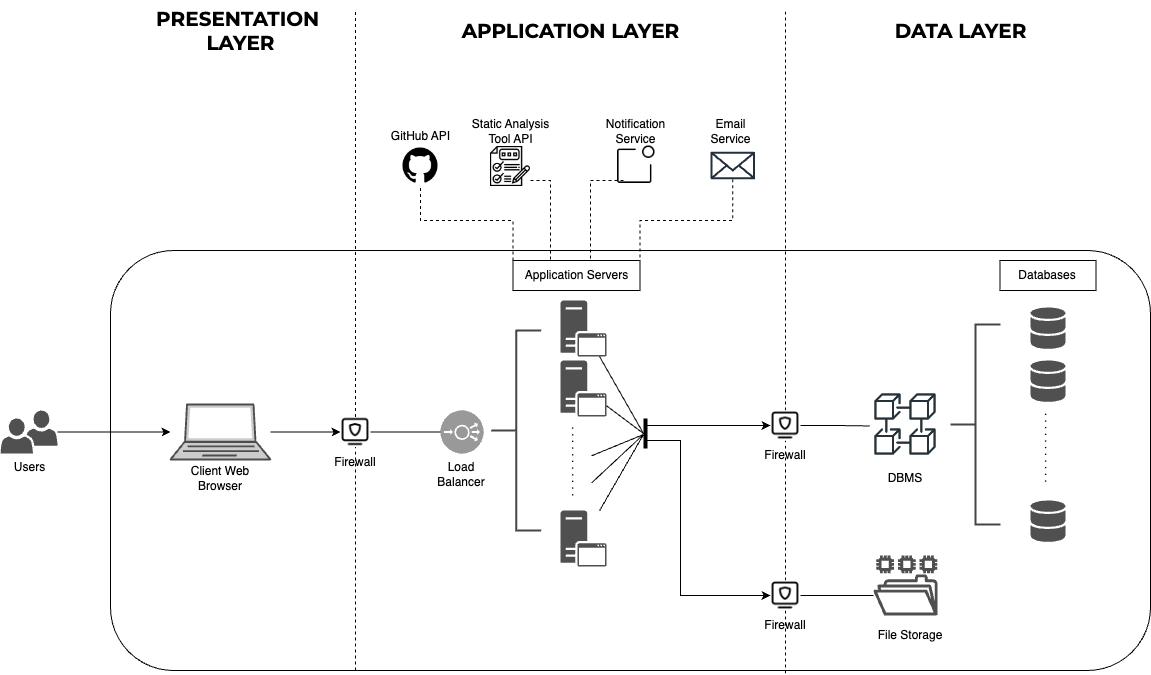
\includegraphics[width=\linewidth]{Images/hl-architecture.drawio.png}
    \caption{High-Level Architecture of the System}
\end{figure}


\subsection{Component View}




\subsection{Deployment View}






\subsection{Runtime View}




\subsection{Component Interfaces}



\subsection{Selected Architectural Styles and Patterns}




\subsection{Other Design Decisions}


